\documentclass{beamer}
\usetheme[color=ACMblue]{ACMNew}
\usepackage{beamernotes}
\usepackage{algpseudocodex}
\usepackage{lipsum}
\usepackage{minted}
\usemintedstyle{manni}
\pdfcompresslevel=9
\pdfobjcompresslevel=3

\title[ACM fun]{CS 438 MT1 Review}
\author{ACM @ UIUC}
%\institute{The Mental Institute}
\date{September 26, 2024}

\begin{document}

\begin{frame}
  \titlepage
\end{frame}
\bnote{This generates notes for pdfpc. These notes also appear
  on the handout/article versions.}

\begin{frame}[t]{Disclaimers and Logistics}
  \begin{itemize}
  \item \alert{Disclaimer:} We have not seen the exam. We have no idea what the questions are. However, we've taken the course and reviewed material/practice exams, so we have \alert{suspicions} as to what the questions will be like.
  \item This review session is being recorded. Recordings and slides will be distributed on Piazza and the ACM site at the end.
  \item \alert{Agenda:} We'll review all topics likely to be covered, working through some examples that may look like exam questions as we go, then review individual topics by request.
  \begin{itemize}
      \item Questions are designed to be written in the same style as previous exams but to be \textit{slightly} harder, so don't worry if you don't get everything right away!
  \end{itemize}
  \item Please let us know if we're going too fast/slow, not speaking loud enough/speaking too loud, etc.
  \item If you have a question anytime during the review session, please ask! Someone else almost surely has a similar question.
  \item We'll provide a feedback form at the end of the session.
  \end{itemize}
\end{frame}

\begin{frame}[t]{Foundations I: Resource Sharing}
 \begin{itemize}
     \item A \alert{network} is just a set of \alert{elements} (servers, routers, etc.) connected together, that implements a set of \alert{protocols} for the purpose of \alert{sharing resources} at the end hosts
     \begin{itemize}
        \item Visualized as graph with elements as nodes and \alert{links} as the edges connecting them
        \item \pause Only one goal- deliver the data between edge nodes
     \end{itemize}
     \item \pause \alert{Statistical Multiplexing}: combining demands to share resources without overbuilding capacity, as aggregate of peak demand is much bigger than peak of aggregate demand. Two approaches:
    \begin{itemize}
        \item \pause \alert{Reservations/Circuit Switching}: Source sends call request, path between source and destination reserved + blocked off, communication happens, then circuit teardown. Used in some telephone + ATM protocols. Can share a channel using FDM (split frequencies) or TDM (round-robin whole resource)
        \item \pause \alert{Packets/Datagrams}: Packets contain data (body) + information on how/where to send it and where it came from (headers). No underutilization/blocked connections/setup costs and can route around link failures, but no guarantees on availiability/delay, and overhead from headers. Used basically everywhere. 
    \end{itemize}
 \end{itemize}    
\end{frame}
\begin{frame}[t]{Foundations II: Internet as IPC}
    \begin{itemize}
        \item Main problem: \alert{inter-process communication}, where processes may not be on the same machine
        \begin{exampleblock}{End-To-End Story}
            \begin{itemize}
                \item \pause Program opens \alert{socket} which allows it to connect to \alert{network stack}
                \item \pause \alert{DNS} maps name of target to \alert{address}
                \item \pause Network stack embeds address and \alert{port} of source/destination in datagram headers
                \item \pause \alert{Routers} create \alert{routing tables} to decide which \alert{outgoing link} to send packets along (knowing only local information). When link is free, forward packet to next router
                \item \pause When packet arrives at destination, forward to correct application
            \end{itemize}
        \end{exampleblock}
        \item Goal: Nodes shouldn't have to worry about the implementation details of other nodes, just the correct decision locally (modularity)
    \end{itemize}
\end{frame}

\begin{frame}{Foundations III: Layering}
    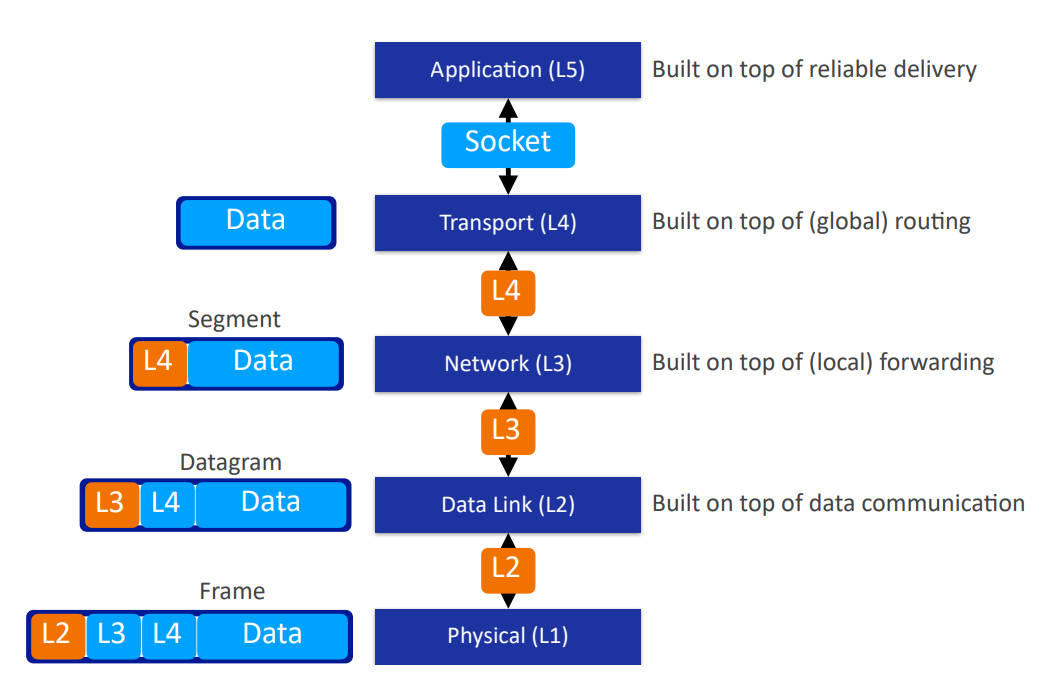
\includegraphics[height=12cm]{layer diagram.png}
\end{frame}

\begin{frame}[t]{Foundations IV: Desiderata}
    \begin{itemize}
        \item \alert{Data Loss}: some applications (video/audio) can tolerate it, others (file transfer/ssh/etc.) can't
        \begin{itemize}
            \item \pause \alert{Packet Error Rate} = $\frac{N}{P}$ for $N$ unrecoverable bit errors for $P$ packets. Packets can be recovered through error-correcting coding, depending on schema. 
            \item \pause Example: if bit error rate is $10^{-6}$, packet 10kb, no ECC, then PER is $1-(1-10^{-6})^{10240} = 1.0\%$
        \end{itemize}
        \item \pause \alert{Bandwidth}: some applications (video streaming) require some amount to be effective, but ``elastic apps'' can use whatever bandwidth they get
        \begin{itemize}
            \item \pause \alert{Throughput}: Number of \textit{total} correctly delivered bits in unit time
            \item \pause \alert{Goodput}: Number of \textit{application-layer} correctly delivered bits in unit time
        \end{itemize}
        \item \pause \alert{Timing}: some applications need packets to be delivered right away (video games/live conferencing/etc.). \alert{Per Packet Latency} = Transmit time + Propagation delay + Process time + Queuing Delay. Assuming packet length $L$, transmit rate $R$ bps
        \begin{itemize}
            \item \pause \alert{Transmit Time}: Time used by transmitter to write packet to wire ($\frac{L}{R}$)
            \item \pause \alert{Propagation Delay}: Time for packet to travel from transmitter to receiver ($\frac{\text{distance}}{\text{velocity}}$)
            \item \pause \alert{Process Time}: Time required for router to read header + decide route
            \item \pause \alert{Queuing Delay}: Time that a packet waits in queue because link is busy. In expectation, proportional to $\frac{La}{r}$ with $a$ packets in queue.
        \end{itemize}
    \end{itemize}
\end{frame}

\begin{frame}[t]{Foundations V: Signal Processing}
\begin{itemize}
    \item \alert{Frequency Band} refers to the range of frequencies used for a signal. \alert{Bandwidth} is the width of this band, is proportional to data rate.
    \item Frequency bands may be divided up into smaller \alert{channels} for simultaneous communication
    \item \pause \alert{Carrier Frequency}: Fixed (higher) frequency used to carry signal. Options include \alert{Amplitude Shift Keying}, \alert{Frequency Shift Keying}
    \item \pause \alert{Signal to Interference and Noise Ratio}: $\frac{P_{\text{signal}}}{P_{\text{noise}}+ P_{\text{interference}}}$. Bit error rate is a function of this. 
    \begin{theorem}[Shannon Capacity]
        $C = B\> \log_2 (1 + SINR)$
        \begin{itemize}
            \item Capacity ($C$) in bits per second
            \item Bandwidth ($B$) in Hz
        \end{itemize}
    \end{theorem}
\end{itemize}
    
\end{frame}

\begin{frame}[t]{Application Layer: Transport Protocols}
\begin{itemize}
    \item Applications can choose between TCP and UDP
    \item \pause TCP
    \begin{itemize}
        \item Uses connection setup between processes
        \item Provides a \alert{reliable transport} guarantee w.r.t. correctness/order/duplication
        \item \alert{Flow control}: sender won't overwhelm receiver
        \item \alert{Congestion control}: Will slow down to avoid network overload
        \item No guarantees on timing, bandwidth
    \end{itemize}
    \item \pause UDP
    \begin{itemize}
        \item Unreliable data transfer between sender and receiver. No fancy control/ordering systems.
    \end{itemize}
    \item \pause Most internet protocols (HTTP/FTP/SMTP/etc.) are built on TCP, but a lot of video streaming/VoIP/trading systems use UDP
\end{itemize}
\end{frame}

\begin{frame}[t]{Application Layer: DNS}
    \begin{itemize}
        \item A \alert{distributed database} implemented as a hierarchy of \alert{name servers} to \alert{resolve} domain names as IP addresses at the application layer
        \begin{itemize}
            \item 13 \alert{root} DNS servers, thousands of TLD DNS servers (.com/.edu/.org/.uk), \alert{authoritative} DNS servers set up by organization or service provider providing an authoritative source for organization's servers (web, mail, etc.)
        \end{itemize}
        \item \pause \alert{Iterative Querying}: Server either returns the record, or an address of a DNS server who might
        \item \pause \alert{Recursive Querying}: Server returns record, asking other servers if needed
        \item \pause When any DNS server learns a mapping, it \alert{caches} it (which times out and disappears eventually). Most common TLD servers are often cached locally, meaning root name server unusual.
        \item \pause 4 types of records: A (hostname \texttt{name} is IP address \texttt{value}), NS (authoritative name server for \texttt{name} can be found at \texttt{value}), CNAME (the ``real'' name for alias \texttt{name} is the canonical name \texttt{value}), MX (the mailserver for \texttt{name} has name \texttt{value})
        \item \pause Inserting Records: Provide registrar with name and IP of authorative name server, registrar inserts NS record for auth server name and A record for auth server IP
        
    \end{itemize}
\end{frame}

\begin{frame}[t]{Application Layer: Architectures}
    \begin{itemize}
        \item \alert{Client-Server}
        \begin{itemize}
            \item Server: always-on host with constant address, Clients: communicate only with servers and not with each other, may disconnect/reconnect, change IP addresses.
        \end{itemize}
        \item \pause \alert{Peer-to-Peer}
        \begin{itemize}
            \item No always-on server, peers might disconnect, change addresses. Scalable, but sometimes difficult to manage. Examples: CHORD, Gnutella
        \end{itemize}
        \item \pause  Many services use hybrid (ex: video conferencing/instant messaging: users directly connect with each other but use central server to register/look up \textit{where} users are)
    \end{itemize}
\end{frame}

\begin{frame}[t]{Application Layer: HTTP}
   \begin{itemize}
       \item Web pages consist of \alert{objects} (HTML, images, javascript, etc.), each of which has a URL
       \item \pause  \alert{HTTP uses a client-server model} where clients request + render, servers send objects in response to requests.
       \item \pause \alert{HTTP uses TCP}. Clients connect to port 80 of host, messages are exchanged between brower + server.
       \item \pause \alert{HTTP is ``stateless''}. Servers maintain no information about previous requests.
       \item \pause \alert{Non-Persistent HTTP} (HTTP/1.0): Connection closes after one response. What's the total response time? \pause \alert{2 $\times$ RTT + file transmit time} per object.
       \item \pause \alert{Persistent HTTP without pipelining}: Connection stays open, but waits for one message response before the next one is sent. What's the total response time? \pause \alert{(\# of referenced objects + 1) $\times$ RTT + data transmit time}
       \item \pause \alert{Persistent HTTP \textit{with} pipelining} (HTTP/1.1 default): Connection stays open, \textit{and} client requests a file as soon as it's referenced. What's the min possible total response time? \pause \alert{Setup + data transmit + 1 RTT for \textit{all} objects}.
   \end{itemize} 
\end{frame}

\begin{frame}[fragile, t]{Application Layer: HTTP}
    \begin{itemize}
        \item Two types of messages: \alert{request}, \alert{response}. Headers in ASCII (except for HTTP/2 or later versions).
        \begin{itemize}
            \item Example Request: {\small \begin{verbatim}
GET / HTTP/1.1
Host: illinois.edu
User-Agent: curl/8.9.1
Accept: */*
            \end{verbatim}}
            \item \pause Method types: GET (gets requested file, can have information in URL parameters), POST (uploads body to server), HEAD (leaves everything but headers out), PUT (uploads file to path in URL field), DELETE (deletes file in URL field)
            \vspace{.5cm}
            \item \pause Example Response: {\small \begin{verbatim}
HTTP/1.1 200 OK
Date: Mon, 21 Oct 2024 23:15:43 GMT
Server: Apache/2.4.57 (Red Hat Enterprise Linux) OpenSSL/3.0.7
Last-Modified: Mon, 23 Sep 2024 21:24:01 GMT
ETag: "eac6-622d001ecb792"
Accept-Ranges: bytes
Content-Length: 60102
Content-Type: text/html; charset=UTF-8
            \end{verbatim}}
        \end{itemize}
    \end{itemize}
\end{frame}

\begin{frame}[t]{Application Layer: Caching}
    \begin{itemize}
        \item \alert{Goal}: Satisfy client request without involving origin server
        \item \pause Browser sends all requests to cache, which acts as both client and server. If cache has file, returns immediately, else requests from server and returns. \alert{Which requests does this help?}
        \item \pause Can use \alert{conditional GET requests}. Add \texttt{If-modified-since} field to headers; if not modified, return status 304, else return file. Ensures that requests are up-to-date while still saving bandwidth. \alert{Why?}
    \end{itemize}
\end{frame}

\begin{frame}[t]{Application Layer: SMTP}
    \begin{itemize}
        \item Uses TCP on port 25 to send mail
        \item Sending mail server acts as ``client'', while recieving server acts as ``server''. This makes it a ``push'' protocol, rather than a ``pull'' protocol (like HTTP)
        \item Three phases of transfer: handshake, message transfer, closure. Commands in ASCII, response is status code + message.
        \item Users access email boxes via \alert{user agents} (POP3/IMAP/webmail).
        \item Lots more details, but they're highly unlikely to come up on an exam.
    \end{itemize}
\end{frame}

\begin{frame}[t]{Application Layer: CHORD}
    \begin{itemize}
        \item Each file assigned a hash and assigned to the next highest node, each server knows a ``finger table'' of nodes exponentially far away from current id, recursive lookup structure.
        
        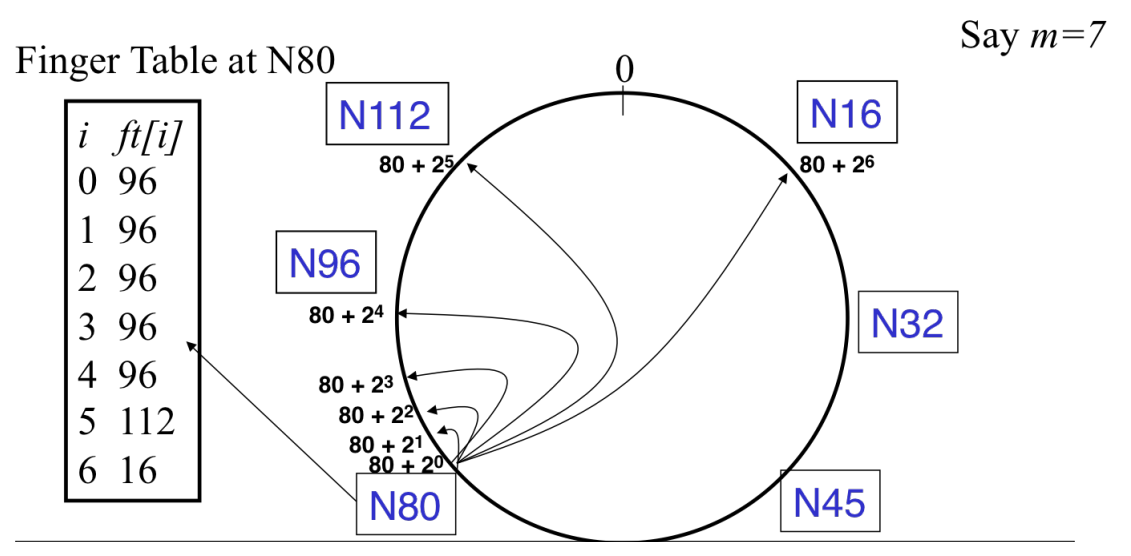
\includegraphics[height=10cm]{chord.png}
    \end{itemize}
\end{frame}


\begin{frame}[t]{Transport Layer: Goals}
    \begin{itemize}
        \item We need to provide a \alert{reliable data stream} to the receiver's application from the sender's application. However, there's a lot that can go wrong:
        \begin{itemize}
            \item \pause Packets can be lost
            \item \pause Packets can arrive out-of-order
            \item \pause Packets can be delayed arbitrarily long
            \item \pause Packets can be duplicated
            \item \pause Packets can be corrupted
            \item \pause We can overwhelm a sending/receiving buffer (thereby dropping packets)
            \item \pause If we transmit too much, we can interfere with other communication going on
        \end{itemize}
        \item \pause We don't want to use any information about lower/higher layers
        \item \pause Also, distributed consensus is \textit{hard}. Some of what we want to do is the \alert{Two Generals' Problem}: since message acknowledgments are as likely to be lost as messages, we'd potentially need infinite messages to come to consensus safely.
    \end{itemize}
\end{frame}

\begin{frame}[t]{Transport Layer: Basic Validation}
    \begin{itemize}
        \item Most protocols: to avoid out of sequence ordering, assign each packet a \alert{sequence number}. Send an \alert{acknowledgment} (ACK) if packet received.
        \item \pause Packets can be corrupted. Receiver can calculate \alert{checksum} to verify validity, as well as run ECCs if protocol provides (Hamming codes, etc.) Some protocols send NACKs to indicate that packet has been rejected, but most just ignore packet. 
        \item \pause Idea: Instead of verifying message/ACK reception, have sender simply resend the packet if no ACK has been received after some time. If receiver receives duplicate packet (by sequence number), acknowledge but throw out. \alert{How does this avoid two generals?} \pause Receiver doesn't know (or care) \textit{which} ACKs have been received, so no distributed consensus.
    \end{itemize}
\end{frame}

\begin{frame}[t]{Transport Layer: Pipelined Protocols}
    \begin{itemize}
        \item Validation + one-packet-at-a-time approach is correct, but is intolerably slow. \alert{Solution:} allow \textit{multiple} packets to be ``in-flight'' (forming a \alert{context window})
        \item \pause \alert{Go-Back-$N$} (GBN): Receiver keeps track of the first packet that has \textit{not} been received (expected\_seq\_num). 
        \begin{algorithmic}[1]
        \Procedure{recieve}{$k$}
            \If{$k$ = expected\_seq\_num}
                \State Send ACK($k$); expected\_seq\_num $\gets$ expected\_seq\_num $ + 1$
            \Else
                \State Send ACK(expected\_seq\_num - 1) \Comment{``cumulative ACK''}
            \EndIf
        \EndProcedure
        \end{algorithmic}
        \begin{itemize}
            \item On timeout: resend \textit{all} packets in CW
        \end{itemize}
        \item \pause \alert{Selective ACK}: receiver individually acknowledges all correctly received packets (ACK($k$)), buffers if needed for in-order delivery to application layer. Sender retransmits packets where no ACK received. If receiver receives a packet with the same sequence number as something in the buffer, throw out.
        \item \pause TCP takes a \alert{hybrid approach}, reports cumulative ACKs (lowest seq \# not recieved - 1), but will accept out-of-order packets and reorder them.
        \begin{itemize}
            \item \pause Sender considers multiple ACK($i$)s as \alert{dupACK}s, fresh $i$ in ACK($i$) \alert{newACK}. Useful for estimating congestion.
        \end{itemize}
    \end{itemize}
\end{frame}

\begin{frame}[t]{Transport Layer: TCP Congestion Control}
    \begin{itemize}
        \item \alert{Main Problem}: How large do we make the context window?
        \begin{itemize}
            \item If too large, then router queues fill up, dropped packets, no fair sharing.
            \item If too small, then suboptimal performance.
        \end{itemize}
        \item \pause Initially, (after SYN/SYN-ACK/ACK), transmitter transmits small burst of packets, waits for ACK. Exponentially increases burst size (\alert{slow start}).
        \item \pause After some point (\alert{SST}/\alert{LIT}), switch from doubling the window size every burst to increasing it by 1 per burst.
        \item \pause Sender keeps a timer to interrupt for timeout. When CW shifted, increase the timer by the gap between packets. On timeout, drastically decrease CW, SST, resend packets.
        \item \pause DupACKs aren't necessarily a bad sign, but might be indicator of missed packets. If 3 dupACKs in a row, retransmit DupACK packet but don't reset SST, slightly cut CW (\alert{fast recovery}).
    \end{itemize}
\end{frame}

\begin{frame}[t]{Transport Layer: TCP State Machine}
    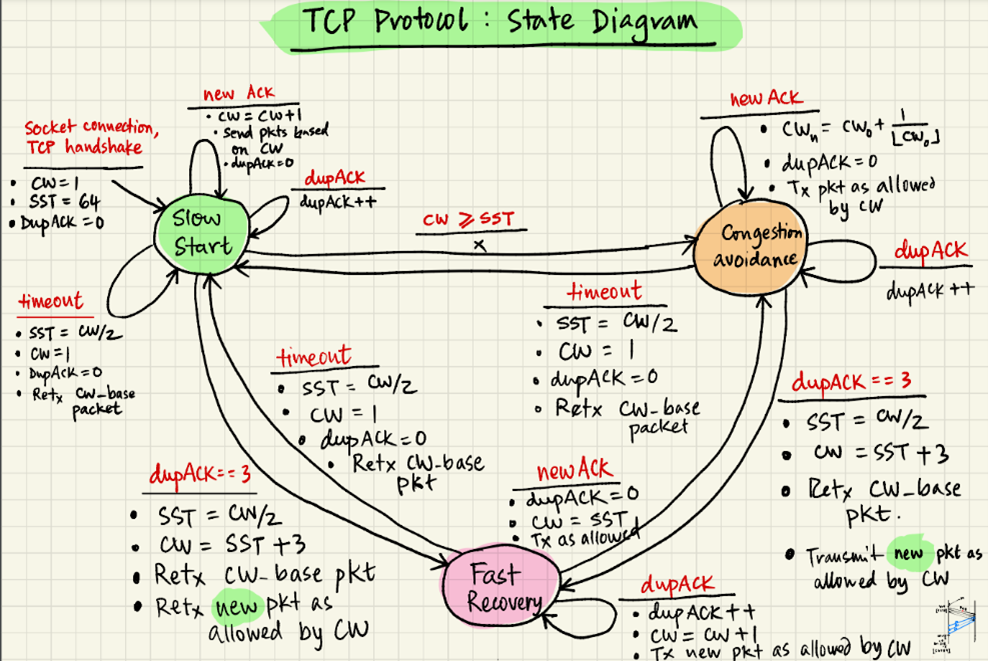
\includegraphics[height=14cm]{tcp flowchart.png}
\end{frame}

\begin{frame}[t]{Transport Layer: TCP RTO Estimation}
    \begin{itemize}
        \item How do we estimate how long timeout (RTO) should be?
        \begin{itemize}
            \item \pause If too short, then premature timeout
            \item If too long, then slow reactions to packet loss
        \end{itemize}
        \item \pause \alert{Intuition}: should be AvgRTT + some ``guard factor''.
        \item \pause AvgRTT estimated by rolling average: $RTT_{avg} \gets (1-\alpha) RTT_{avg} + \alpha\> RTT_{packet}$
        \item \pause ``guard factor'' can be a deviation estimate: \begin{align*}
            devRTT_{avg} &\gets (1-\beta)\> devRTT_{avg} + \beta (|RTT_{packet} - RTT_{avg}|)\\
            RTO &\gets RTT_{avg} + 4\>devRTT_{avg}
        \end{align*}
    \end{itemize}
\end{frame}

\begin{frame}[t]{Transport Layer: Flow Control and Fairness}
    \begin{itemize}
        \item \alert{Problem}: Receiver has a limited buffer. If many nodes transmitting to same receiver, losses may happen at receiver
        \item \pause \alert{Solution}: Receiver reports how much space left to sender in ACKs. Sender will deliberately use a smaller congestion window (while calculating CW as normal).
        \vspace{1cm}
        \item \pause TCP guarantees \alert{max-min fairness} (in stable state): All flows requesting less than fair share get their request. Remaining flows divide equally.
    \end{itemize}
\end{frame}

\begin{frame}{Feedback}
    \begin{center}
        
\includegraphics[height=12cm]{feedback.png}
        http://go.acm.illinois.edu/cs438\_mt1\_feedback
    \end{center}
\end{frame}
\end{document}
